\documentclass{beamer}

\usepackage{amsmath}
\usepackage{amssymb}
\usepackage{framed}

\begin{document}
\section{Part 1}

\begin{frame}
%---------------------------------------------------- %
\begin{figure}
\vspace{1cm}
\centering

\includegraphics[width=0.7\linewidth]{./RlogoMAM}

%\label{fig:RlogoMAM}
\end{figure}
\LARGE
\[ \mbox{Shiny Demonstration}  \]
\Large


\[ \mbox{30th October 2013}  \]
\end{frame}
%---------------------------------------------------- %
\begin{frame}
\begin{figure}
\Large
\centering

\includegraphics[width=0.55\linewidth]{./Rstudio}
\[ \mbox{rstudio}  \]
%\label{fig:RlogoMAM}
\end{figure}

\end{frame}
\begin{frame}
%--------------------------------------------------%
\frametitle{RStudio}
\LARGE
\begin{itemize}
\item Makers of Shiny : RStudio\\ (JJ Allaire, Hadley Wickham etc etc)
\item RStudio? IDE for \texttt{R}. See \texttt{www.rstudio.org} for more.
\item Shiny's  Lead Developers : Winston Chang and Joe Cheng.
\end{itemize}

\end{frame}
%---------------------------------------------------- %
\begin{frame}
\frametitle{Shiny - Slides Set 1}
\Large
\begin{itemize}
\item Some Announcements
\item Overview of Demonstration
\item Resources (i.e. Shiny Tutorial Page)
\item Minimal Examples 
\item Widgets
\item A bit about JavaScript
\item Deploying Shiny
\end{itemize}
\end{frame}
%---------------------------------------------------- %
%---------------------------------------------%
\begin{frame}
\frametitle{London R - December Meeting}

\begin{description}
\item[Date:]  Tuesday 3rd December

\item[Time:]  6pm (presentations begin at 6.30pm)

\item[Venue:]  Balls Brothers, Minster Pavement, Mincing Lane, London EC3R 7PP
\item[Info:] See \texttt{www.LondonR.org} for more details.
\end{description}
%-----------%
\textbf{Presentations:}
\begin{description}
\item[Andy South] - Making beautiful world maps with country-referenced data using rworldmap and other R packages
\item[Malcolm Sherrington] - Algorithmic Trading with R
\item[Chris Beeley] - Shiny happy web interfaces - Shiny, HTML, CSS, JavaScript, and Shiny Server working together
\end{description}
\end{frame}

%---------------------------------------------%
%---------------------------------------------------- %
\begin{frame}
\Large
\frametitle{What is Shiny?}
\textbf{Easy web applications in R}\\
\textit{(Source: Shiny's Website)}
\begin{itemize}
\item \textbf{\textit{Shiny}} makes it super simple for \texttt{R} users like you to turn analyses into interactive web applications that anyone can use. \item Let your users choose input parameters using friendly controls like sliders, drop-downs, and text fields. \item Easily incorporate any number of outputs like plots, tables, and summaries.
\end{itemize}
\end{frame}
%---------------------------------------------------- %
%---------------------------------------------------- %
\begin{frame}
\Large
\frametitle{What is Shiny?}
\vspace{-1cm}
\textbf{Easy web applications in R (contd.)}\\
\textit{(Source: Shiny's Website)}
\begin{itemize}
\item No \textbf{HTML} or \textbf{JavaScript} knowledge is necessary. If you have some experience with \texttt{R}, you’re just minutes away from combining the statistical power of \texttt{R} with the simplicity of a web page.
\item \textit{(Remark: They do appear to be really handy - based on several examples  available on the internet!)}
\end{itemize}

\end{frame}
%---------------------------------------------------- %


%---------------------------------------------------- %
\begin{frame}
\Large
\frametitle{Shiny Resources}
\vspace{-1.5cm}
\textbf{Resources}
\begin{itemize}

\item Shiny Tutorial (\texttt{http://rstudio.github.io/shiny/tutorial})
\item Chris Beeley's New Book\\ (Sample Chapter Available)
\item Stack-Overflow and GitHub 
\end{itemize}

\end{frame}
\begin{frame}
%---------------------------------------------------- %
\begin{figure}
\vspace{0.5cm}
\centering
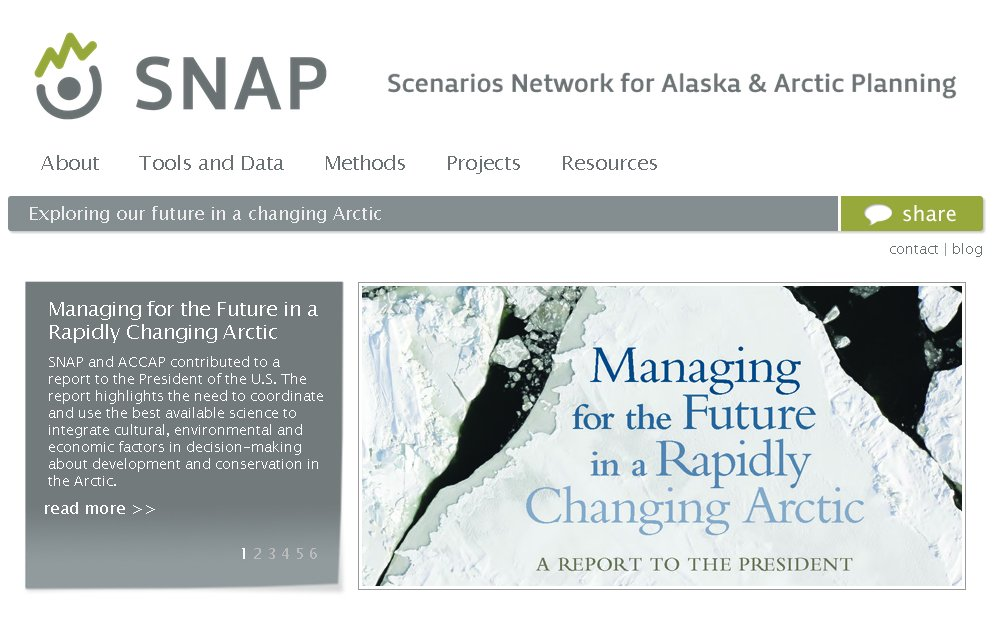
\includegraphics[width=0.75\linewidth]{./snap2}

%\label{fig:RlogoMAM}
\end{figure}
\Large
\[ \mbox{Matthew Leonawicz (SNAP - Uni. Alaska Fairbanks)}  \]
\[\mbox{github.com/ua-snap/shiny-apps}‎\]
\[ \mbox{twitter.com/leonawicz} \]

\end{frame}

%---------------------------------------------------- %
\begin{frame}
\begin{figure}

\centering

\includegraphics[width=0.55\linewidth]{./github}
\[ \mbox{github - code sharing}  \]
%\label{fig:RlogoMAM}
\end{figure}
\Large


\end{frame}





\end{document}
%---------------------------------------------------- %
%\section{Introduction}


\begin{figure}
\centering

\includegraphics[width=0.65\linewidth]{./github}

%\label{fig:RlogoMAM}
\end{figure}
\Large
\[ \mbox{GitHub}  \]

\end{frame}
